% 17-19(본책 17쪽) — 가로 4칸·세로 4칸 도로망 한가운데를 호수(하늘색 얼룩)가 덮어 가운데 교차점으로는 지날 수 없는 그림. A 왼쪽 위 · B 오른쪽 아래. 스캔 그림을 TikZ 로 다시 그림(스캔 화질 · 호수는 원문처럼 가운데 교차점과 그 둘레 네 도로만 덮는다 · 윤곽 모양은 스캔과 똑같지 않다).
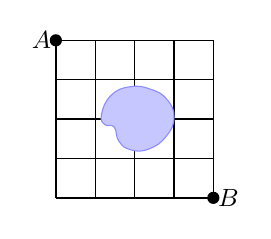
\begin{tikzpicture}[line width=0.5pt]
  \foreach \x in {0, 0.5, 1, 1.5, 2} { \draw (\x,0) -- (\x,2); }
  \foreach \y in {0, 0.5, 1, 1.5, 2} { \draw (0,\y) -- (2,\y); }
  \fill[blue!22, draw=blue!45, line width=0.4pt]
    plot[smooth cycle, tension=0.8] coordinates
    {(0.58,1.06) (0.70,1.30) (0.94,1.41) (1.20,1.38) (1.41,1.25) (1.50,1.02)
     (1.40,0.78) (1.18,0.62) (0.95,0.61) (0.80,0.72) (0.74,0.90) (0.62,0.93)};
  \fill (0,2) circle (2.2pt);
  \node[left, font=\small, inner sep=1.5pt] at (0,2) {$\pt{A}$};
  \fill (2,0) circle (2.2pt);
  \node[right, font=\small, inner sep=1.5pt] at (2,0) {$\pt{B}$};
\end{tikzpicture}
